\section{Method}
\label{sec:mainsub_method}

We present here our approach, which consists of using a simple \gls{vqa} model with a training protocol that encourages consistency among pairs of perception and reasoning questions. Fig.~\ref{fig:method_mainsub} illustrates this \gls{vqa} model and our training approach.

\subsection{VQA Model} Following~\cite{cadene2019rubi}, our \gls{vqa} model,~$f:\mathcal{I}\times\mathcal{Q}\to \mathcal{P}(\mathcal{A})$, takes a tuple containing an image,~$\x$, and a question,~$\q$, to produce a distribution,~$\p=f(\x,\q)$, over a finite set of possible answers~$\mathcal{A}$ (see Fig.~\ref{fig:method_mainsub}(Top)). After encoding the inputs, the \gls{vqa} model combines visual ($v$) and textual ($q$) features through an attention module ($k$)~\cite{xu2015show} that selects the visual features relevant to the question ($v'$). The final classifier receives a combination of the relevant features and the text features through a fusion module to predict the final distribution.

In some cases, questions may be asking about content related to specific regions of the image (\eg, ``are there hard exudates in this region?''). To process these cases, the input image is masked so that the visible area corresponds to the region mentioned in the question while the rest of the image is set to zero.

Training this model requires a dataset~$\mathcal{T}=\{t^{(i)}=(\x^{(i)}, \q^{(i)}, a^{(i)})\}_{i=1}^N\subseteq\mathcal{I}\times\mathcal{Q}\times\mathcal{A}$ of images and questions annotated with their answers. The \gls{vqa}~loss is simply the cross-entropy between the predicted distribution and the real answer,
\begin{equation}
    \label{eq:vqa_loss}
    \ell_{\textrm{VQA}}(\p, a) = H(\p, a) = -\log \p_a.
\end{equation}
While this loss alone is sufficient to reach a reasonable performance, it ignores the potentially useful interactions that may exist among training questions.
\begin{figure}[!h]
\begin{center}
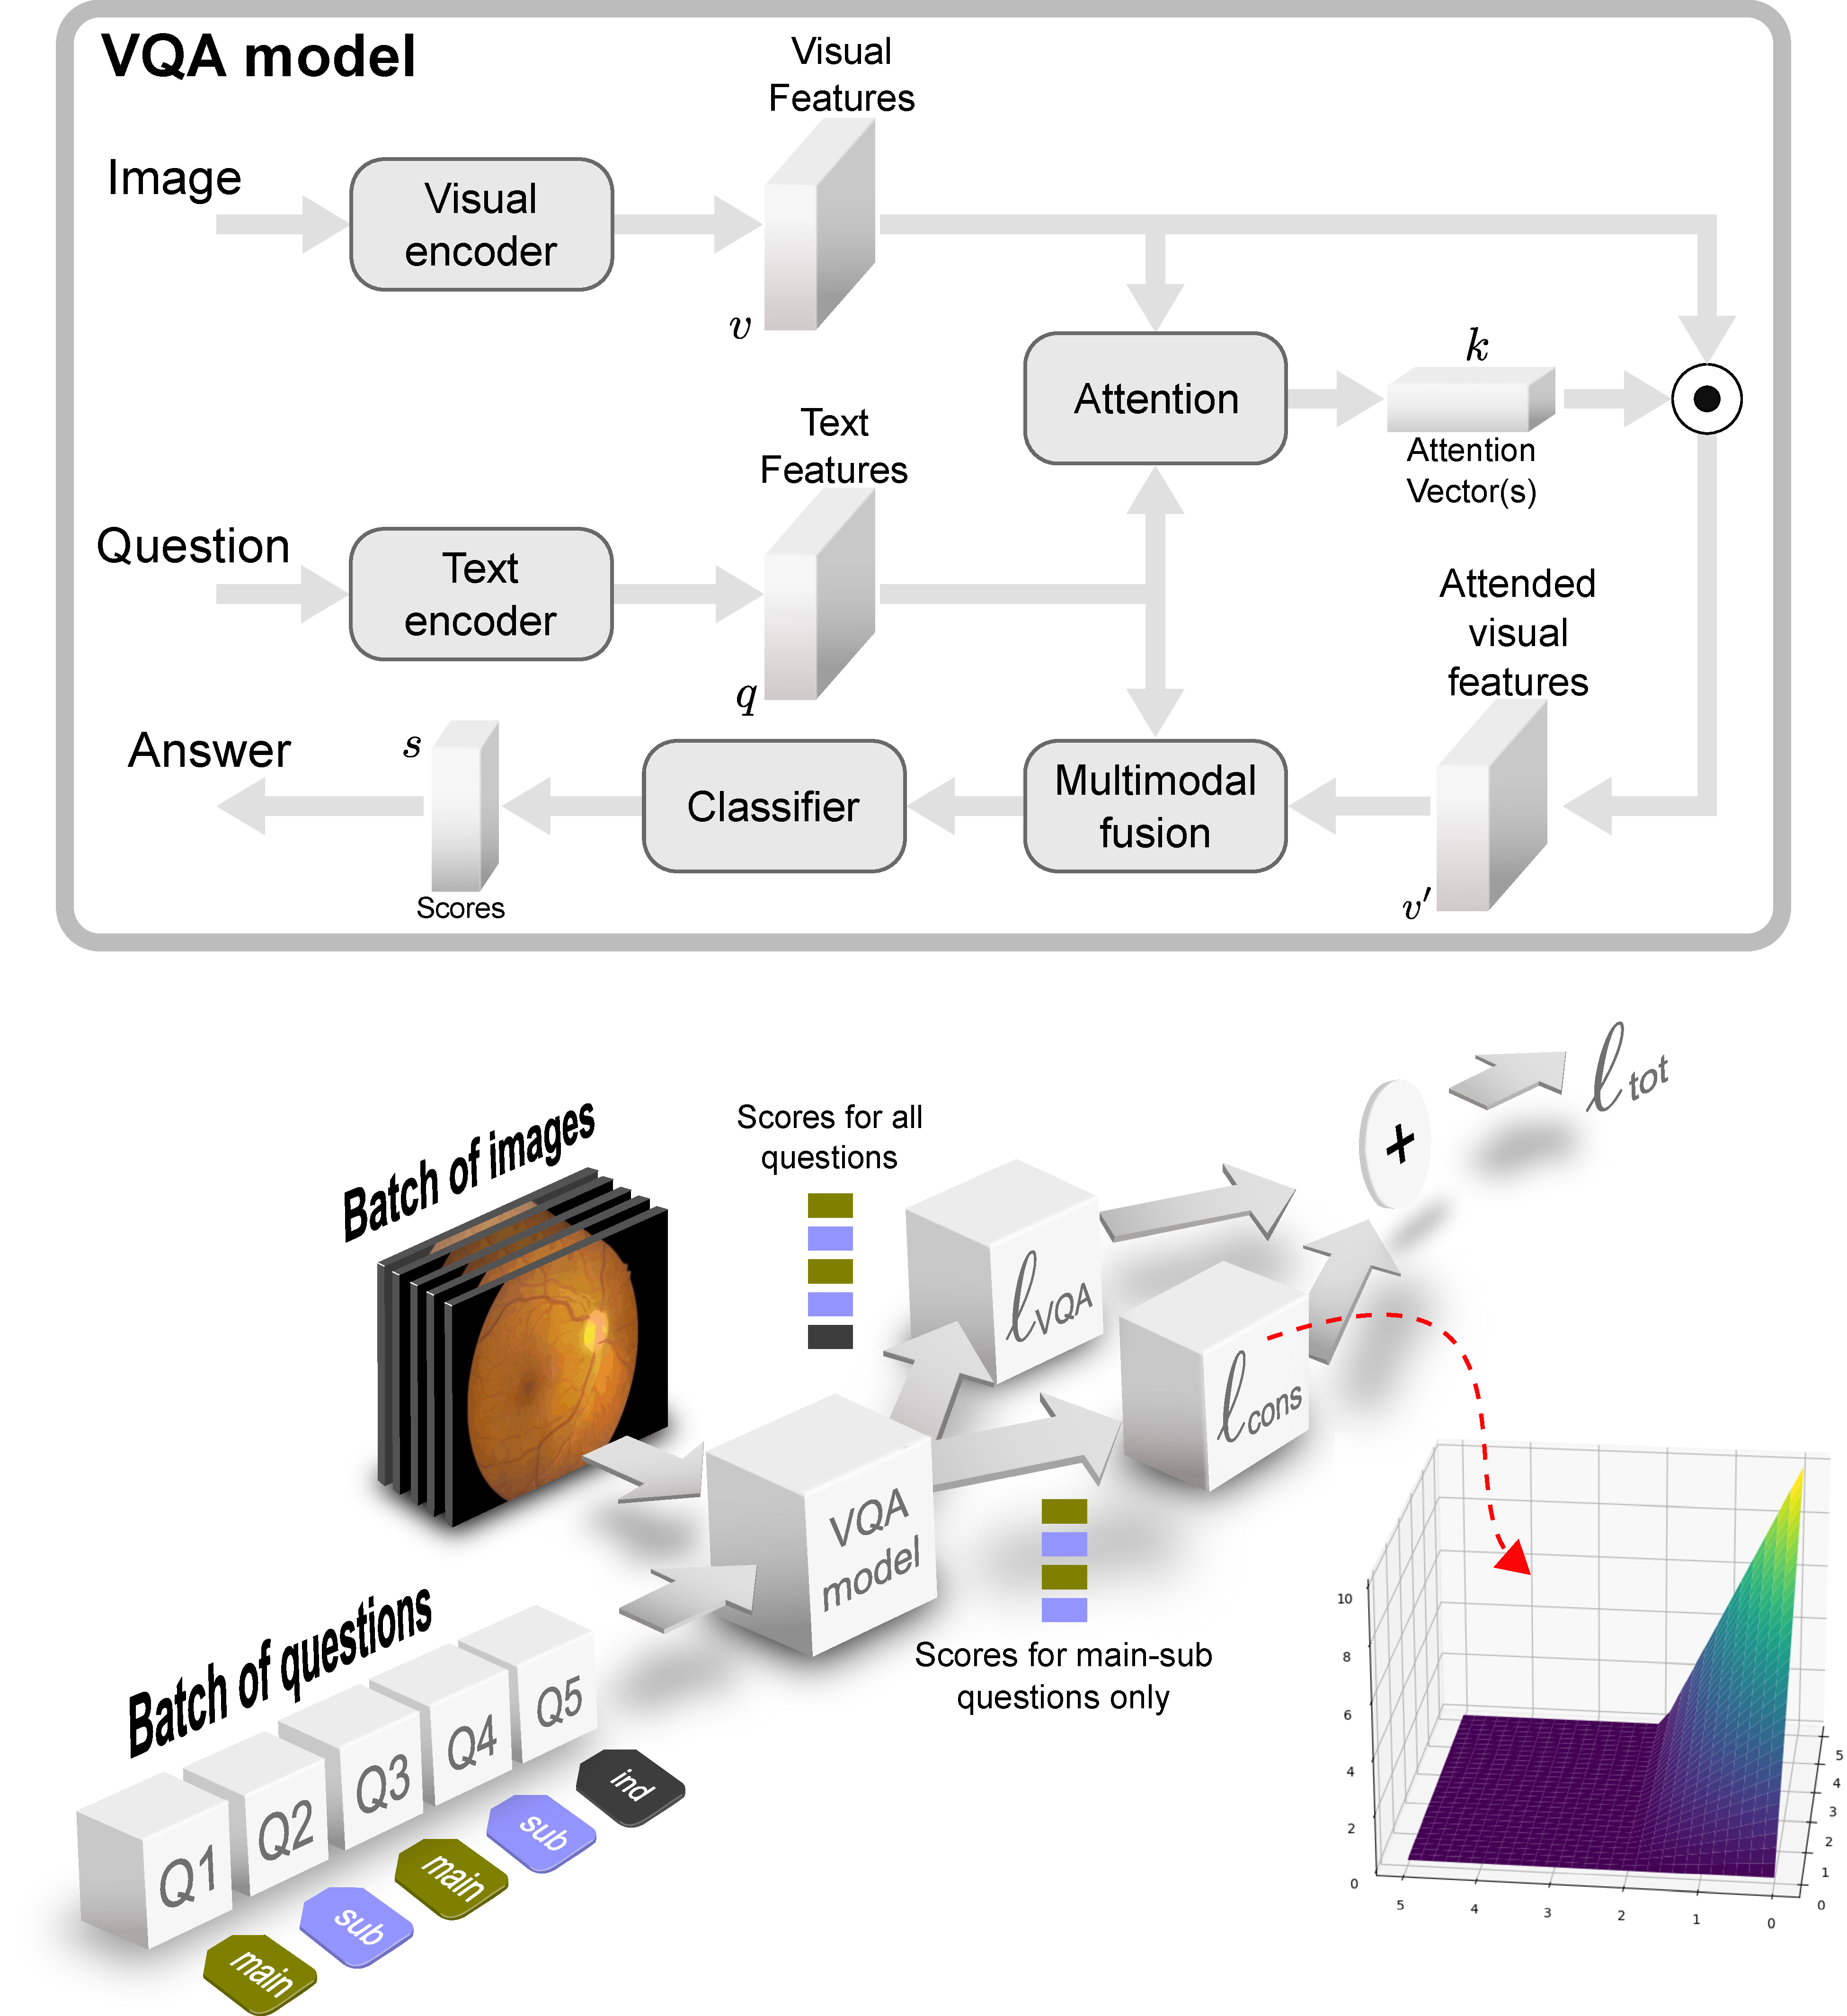
\includegraphics[width=0.75\textwidth]{Figures/Part2_Consist/01_mainsub/method.pdf}
\caption{\textbf{Top:} VQA model architecture. \textbf{Bottom:} Visualization of the training process with the proposed loss. The total loss, $\ell_{\textrm{tot}}$, is based on two terms: the conventional VQA loss,  $\ell_{\textrm{VQA}}$ and our proposed consistency loss term, $\ell_{\textrm{cons}}$. The latter is computed only for pairs of main (reasoning) and sub (perception) questions. Training mini-batches consist of main and sub-questions at the same time, whereby sub-questions can consider specific regions of the image. Unrelated questions (denoted with ``ind") can also be included in training batches but do not contribute to $\ell_{\textrm{cons}}$.}
\label{fig:method_mainsub}
\end{center}
\end{figure}


\subsection{Consistency Loss} We aim to improve the quality of our \gls{vqa} model by exploiting the relationships between reasoning and perception questions at training time. To this end, we augment the training dataset with an additional binary relation~$\prec$ over the set of questions~$\mathcal{Q}$. Two questions are related, $\q^{(i)}\prec \q^{(j)}$, if $\q^{(i)}$ is a perception question associated to the reasoning question~$\q^{(j)}$. From hence on, we refer to perception questions as \emph{sub-questions} and reasoning questions as \emph{main questions}.

Following the terminology in~\cite{selvaraju2020squinting}, an inconsistency occurs when the \gls{vqa} model infers the main question correctly but the sub-question incorrectly. Using the entropy as a measurement of incorrectness, we propose to impose the consistency at training time by penalizing the cases with high $H^{(i)}=H(\p^{(i)}, a^{(i)})$ and low $H^{(j)}=H(\p^{(j)}, a^{(j)})$ when $\q^{(i)}\prec \q^{(j)}$. To do this, we use an adapted hinge loss that disables the penalty when $H^{(j)}$ is larger than a threshold~$\gamma>0$, but otherwise penalizes large values of~$H^{(i)}$,
\begin{equation}
    \label{eq:cons_loss}
    \ell_{\textrm{cons}}(H^{(i)}, H^{(j)}) = H^{(i)}\max\{0, \gamma - H^{(j)}\}.
\end{equation}
\noindent
%$\gamma \in \mathbb{R}^+$. Fig.~\ref{fig:method_mainsub}(Bottom) illustrates $\ell_{\textrm{cons}}$. 

The final cost function then minimizes the expected value of the \gls{vqa} loss~\eqref{eq:vqa_loss} for the elements of the training dataset and the consistency loss~\eqref{eq:cons_loss} for the pairs of training samples with $\prec$-related questions,
\begin{equation}
    \label{eq:cost}
    \mathbb{E}_{t\sim\mathcal{T}}[\ell_\textrm{VQA}(\p, a)] +
    \lambda\mathbb{E}_{(t^{(i)}, t^{(j)})\sim\mathcal{T}^2}[\ell_\textrm{cons}(H^{(i)}, H^{(j)}) \mid \x^{(i)}=\x^{(j)}, \q^{(i)}\prec\q^{(j)}],
\end{equation}
where $\lambda > 0$ controls the relative strength of both losses and $\mathcal{T}^2$ is the Cartesian product of $\mathcal{T}$ with itself, that is, all pairs of training samples.

To train, this cost is iteratively minimized approximating the expectations with mini-batches. The two expectations of Eq.~\eqref{eq:cost} suggest that two mini-batches are necessary at each iteration: one mini-batch sampled from~$\mathcal{T}$ and a second mini-batch of $\prec$-related pairs sampled from $\mathcal{T}^2$. However, in practice a single mini-batch is sufficient as long as we ensure that it contains pairs of $\prec$-related questions. While this biased sampling could in turn bias the estimation of the first expectation, we did not observe a noticeable impact in our experiments. Fig.~\ref{fig:method_mainsub}(Bottom) illustrates this training procedure.